\chapter{Exploring the maths library through the CPP Reference}\label{chp:maths}
\epigraph{Do not worry about your difficulties in Mathematics. I can assure you mine are still greater.}{Albert Einstein}

Many common problems for programming in C are already solved and compiled into a \emph{standard library}. In this chapter, rather than going through the many functions provided by this library, I will show you how to find out what functionality the C standard library provides and how to use it. In particular, we will focus on the maths library, which offers tools for doing maths (like computing the square root or sine of a number). This part of the standard library was chosen for two reasons: for one, the purpose and usage of these functions can be well understood at our current level of knowledge. Secondly, using these functions requires an extra step when compared to the other functions that I want to show and explain here.

\section{Recap: Headers, Libraries and Linking}
By now we know well enough that machine language does not contain any code that a human could make sense of. Variable names are all gone in favour of naked memory addresses. When we write our code and use precompiled functions like \texttt{printf}, the computer needs to be able to \emph{link} the machine language output of our code with the precompiled binary instructions from the library. That is the end to which a \emph{header} serves: it is a file containing some C code that fills in the gaps between precompiled library and own code. The details of this we will discuss in chapter \ref{chp:modules}. In the case of the maths library, this header is called \texttt{math.h},

But where does the library itself come from? In the case of the \emph{standard} library, the compiler is simply configured to always include this library into the linking process. When we installed the compiler, we also copied the standard library into a  predefined directory which is \enquote{known} to the compiler. Hence, linking can take place with no additional information; all needed file paths are implicitly given.

All other libraries must be specified explicitly to the compiler with the flag \texttt{-l<libname>}\footnote{again, there is an implicitly given path where these libraries are looked for, but we can in principle also specify an absolute file path.}. So, if we want to use \texttt{libcurl}\footnote{Taken from \url{https://curl.se/libcurl/}:\\
\emph{libcurl is a free and easy-to-use client-side URL transfer library, supporting DICT, FILE, FTP, FTPS, GOPHER, GOPHERS, HTTP, HTTPS, IMAP, IMAPS, LDAP, LDAPS, MQTT, POP3, POP3S, RTMP, RTMPS, RTSP, SCP, SFTP, SMB, SMBS, SMTP, SMTPS, TELNET and TFTP.}}, we need to invoke the compiler with the flag \texttt{-lcurl} (provided the library is installed in the first place).

The maths routines are considered part of the standard library; however, they are not given in the same file as the other routines of the standard library. The reason for this is that they are not needed in as many projects as the \enquote{true} standard library, and putting them into a separate file allowed to speed up compilation time, which was useful mostly in the old days of computer science. In order not to break existing workflows, the split stayed up to the modern days.

The main takeaway from all this is: When we want to use maths functions, we need to
\begin{itemize}
\item \texttt{\#include <math.h>}
\item Link with the \texttt{-lm} flag
\end{itemize}


\section{Structure of Articles on cppreference.com}
The website \url{https://en.cppreference.com/w/c} hosts a community-driven reference of all commands and functions of the C standard library. That means that, much like with wikipedia, hobbyists come together and create and maintain this website. It has become an indispensable tool in software devellopment and serves both, private and professional coders alike with high quality content. By default, you will see the English version of the page, which should look like shown in figure \ref{fig:cpp-home}. There are also versions in other languages (cf bottom of the page), but they are often lacking\footnote{In my experience, this is a general trend in the coding world: the best ressources are available in English. While not always their mother tongue, all good programmers speak English at least reasonably well and rather pool their ressources rather than wasting time on translating the same content over and over.}, and are sometimes machine-translated or incompletely translated.

\begin{figure}
	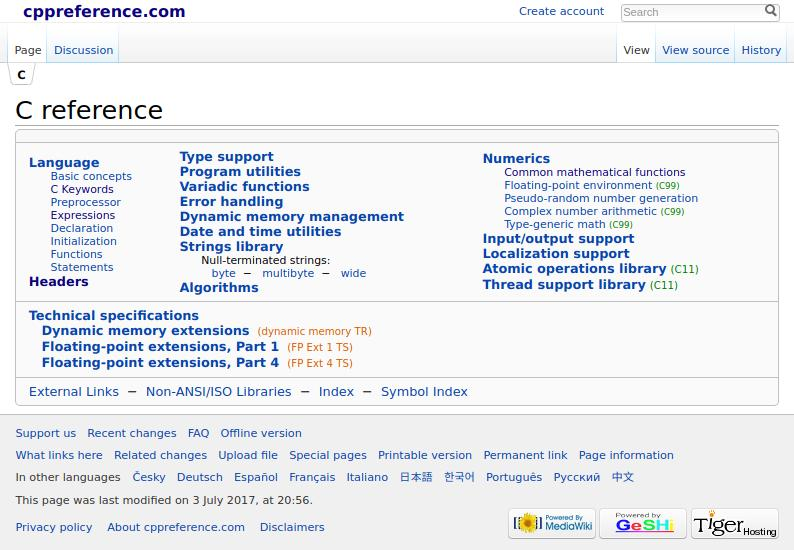
\includegraphics[width=\linewidth]{./gfx/cpp-home}
	\caption{The website \url{https://en.cppreference.com/w/c}} \label{fig:cpp-home}
\end{figure}

In the upper right corner you will find a textbox that allows you to enter a search term. Use this if you need to remember the exact syntax of a command or a detailled description of its effects and limitations. The search function will actually lead you to a \url{duckduckgo.com} search on the site, which means that you can also enter search terms such as \emph{inverse cosine} and are still likely to find what you are looking for without knowing the exact name of the command\footnote{The website has a deprecated search engine of its own which, in my opinion, is nicer to use if you know what you are looking for and only want to read up on specifics of a call. However, the index of this internal search page is no longer maintained, \ie you will not find any pages added to the website after ca. 2018, and your search term must be rather specific. Anyway, if you open up \url{https://en.cppreference.com/mwiki/index.php?title=Special:Search&search=yourSearchTerm}, you can still access it (replace \texttt{yourSearchTerm} with what you are looking for). I still have my browser configured such that I can access the old engine by simply typing \texttt{cpp mySearchTerm} in the address bar.}.

\begin{figure}
	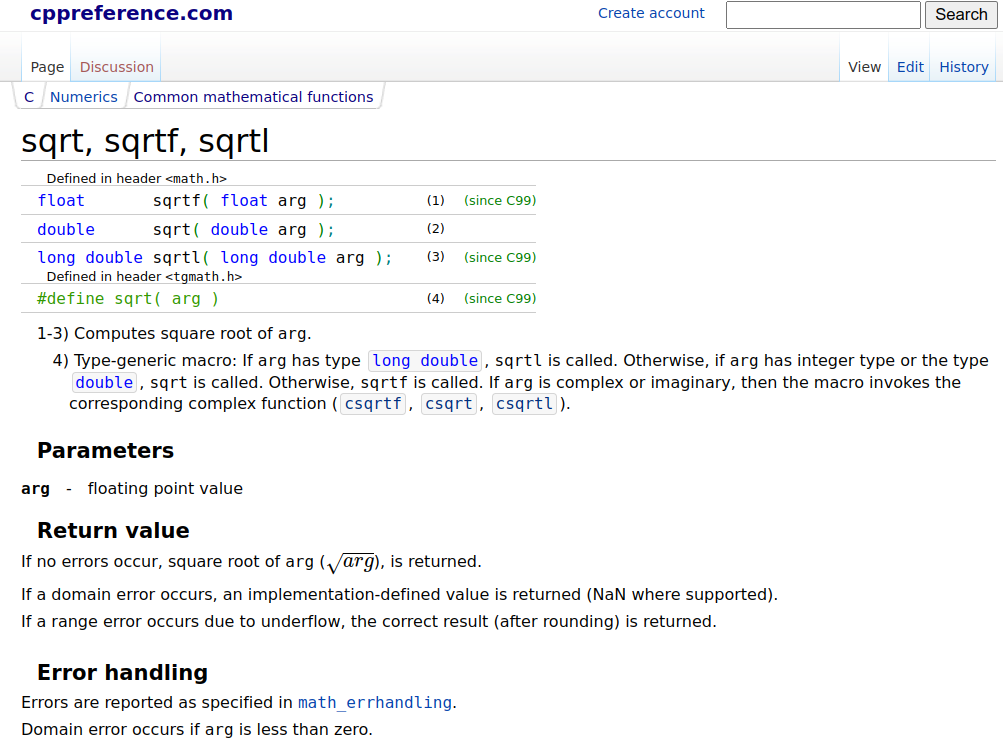
\includegraphics[width=\linewidth]{./gfx/cpp-sqrt}
	\caption{The article for \texttt{sqrt}, \texttt{sqrtf} and \texttt{sqrtl} in the CPP Reference} \label{fig:cpp-sqrt}
\end{figure}

Following these search results, you will get to a page like the one shown in figure \ref{fig:cpp-sqrt}. As you can see, the headline of the article lists several commands that are very similar in use and result. Directly below the headline you find the text \emph{Defined in header \texttt{<math.h>}}, which tells you that to use either of these commands you will need to \texttt{\#include} this header.

Below that, as the first bigger block in the article, you will find a tabular overview over the commands described in the article. In this case you can see that the \emph{return type} of \texttt{sqrtf} is \inC{float} while that of \texttt{sqrt} is \inC{double}. Likewise, they all take one argument, which has a different type depending on the command used.

As mentioned a number of times before, the language C has evolved over the years, and different standards are available. For example, the command \texttt{sqrtf} was only introduced in the revision from 1999. This is hinted at by the green text \emph{since C99}. Sometimes, commands are removed or their use changes. In that case, you will find a note saying \emph{since C...} and possibly multiple lines showing the various versions of the command in the different revisions of the language.

Right before the green marks, you see numbers in parentheses. These are referred to by the text right below the tabular overview. You see the line \emph{1-3) Computes the square root of \texttt{arg}}. So all of these three commands are used to compute square roots; the sole difference between them is the data type of the arguments and the return type. There is also a version (4) which is a bit more difficult to understand at this point, so we will defer that to when we are more familiar with all the features of the C language.
 
Most commands take more than one argument (think of \texttt{printf} for example). So to clarify the meaning of each argument, there's the section \emph{Parameters}, which in this trivial case is only a stub. The section \emph{Return value} informs you not only that in fact $\sqrt{arg}$ is computed, but also what will happen if errors occur. For example, the square root of negative numbers does not exist\footnote{or rather: is not part of the real numbers. You can actually do complex math in C, but we'll discuss that later.} Such a \emph{domain error} results in a \emph{NaN} -- not a number. Think of this as a special bitpattern that only represents a computation gone wrong.

At the end of most articles, you will find an example code together with the output produced by that code (not depicted in \ref{fig:cpp-sqrt}). The commands used in these examples are usually hyperlinked to the articles describing them in detail; so if you encounter commands you do not know yet, you can click on them to directly find a detailled description.

You see that at our current level of knowledge, you will encounter a number of concepts that we haven't discussed yet. Still, we already profit a lot from this tool. You can do both, look up commands that we've already discussed as well as discover new ones and understand how to use them. For example, we now have no longer any problems understanding the following:

\begin{codebox}[squareRoot.c]
\begin{minted}[linenos]{c}
#include <math.h>

int main () {
   double number = 81.0;
   double root = sqrt(number);
   printf("The square root of %lf is %lf.\n", number, root);
}
\end{minted}
\captionof{code}{Computing the square root of a number}
\end{codebox}
In particular, we not only know that \texttt{sqrt} computes the square root of a number, but we also know which data type it expects and which data type it returns. That is, in the above example, we know that no implicit type conversion happens, which eliminates one common source of errors.

With this, I want to encourage you to look up and discover the details for these functions
{
	\newcolumntype{C}{>{\ttfamily\centering\arraybackslash} p{.2\linewidth}}
	\newcolumntype{D}{>{         \centering\arraybackslash} p{.7\linewidth}}
	\rowcolors{1}{white}{tabhighlight}
\begin{center}
\begin{tabularx}
	{.95\linewidth}
	{CD}
\toprule[1pt]

	\normalfont Function  &  Return value
\tabcrlf

	sqrt  & Square root \\
	cbrt  & Cubic root   \\
	pow   & Power of a number \texttt{x} to an exponent \texttt{y}: $x^{y}$ \\
	exp   & Exponential $e^x$ \\
	log   & Natural logarithm \\
	sin   & Sine \\
	cos   & Cosine \\
	tan   & Tangent \\
	asin  & Arc sine \\
	acos  & Arc cosine \\
	atan  & Arc tangent \\
	atan2 & Arc tangent with distinction of quadrants \\
	ceil  & Ceiling function (round upwards to next integer) \\
	floor & Floor function (round down to next integer) \\
	trunc & Truncate decimal part\\
	round & Round number \\

\bottomrule[1pt]
\end{tabularx}
\end{center}
\captionof{table}{Common functions in the math-library}\label{tab:CommonMathFuncs}
}


\section{Finding Functions for a Specific Task}
We already know about the search bar installed on the website. We do not always know the term we are looking for. In such a scenario, we can make use of the fact the the C standard library is grouped thematically in different \emph{headers}, \ie files that we can load into our program with a corresponding \texttt{\#include} directive. We know about \texttt{stdio.h} which handles input and output to our program and \texttt{math.h}, which provides us with mathematical functions. Clicking on the link \href{https://en.cppreference.com/w/c/header}{\texttt{Headers}} on the main page (cf. figure \ref{fig:cpp-home}) brings us to a list of all header files documented in the CPP Reference (cf. figure \ref{fig:cpp-headers}), together with a brief description for the functions provided by the listed header file. For example, we see that a file \texttt{complex.h} allows us to do maths with complex numbers.

\begin{plusbox}[Complex Numbers]
If you do not have a STEM background (science, technology, engineering, maths), complex numbers may be unfamiliar to you. We will not discuss them in much detail here, because this doesn't provide us with much insight into the world of programming. Those who know \emph{what} to use complex numbers for will have no problem learning \emph{how} to use them with the articles in the CPP Reference. Those who have not heard about them yet need not be bothered by higher maths.

If you are curious nonetheless: one can construct a set of \enquote{extended computation rules} when you assume there is a number \textsl{i} that is the solution to $\sqrt{-1}.$ This number \textsl{i} may be added to any real number $a$ or be multiplied with any real number $b$, to form \emph{complex numbers} of the form $z = a + b\textsl{i}$. From this, a whole set of rules for computing can be deduced, starting from addition, subtraction, multiplication and division of complex numbers, up to advanced maths functions like the logarithm or trigonometric functions. In particular, complex numbers eventually lead to \emph{Euler's Formula}:
\[ \exp(\textsl{i} \alpha) = \cos(\alpha) + \textsl{i} \sin(\alpha) \]
which is the generalized form of the \emph{Euler identity}, often called \emph{the most beautiful equation of mathmatics}:
\[ \exp(\textsl{i} \pi) + 1 = 0 \]
\end{plusbox}

\begin{figure}
	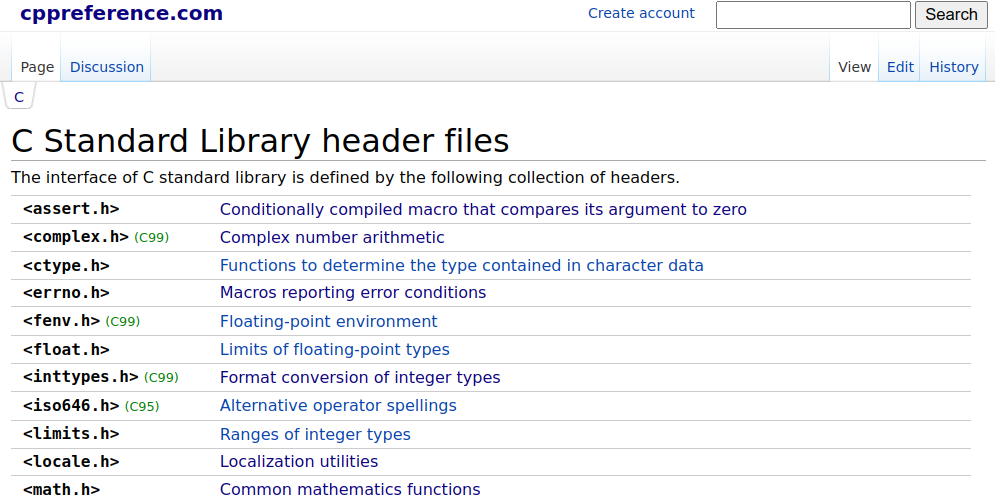
\includegraphics[width=\linewidth]{./gfx/cpp-headers}
	\caption{Part of the header files documented in the CPP Reference} \label{fig:cpp-headers}
\end{figure}

Again, I invite you to have a look at the \href{https://en.cppreference.com/w/c/header}{\texttt{Headers}} section of the CPP Reference and get a feeling of what features are hidden under the surface before we continue our guided tour through the world of C programming.


\section{C++}
The abbreviation CPP stands for C plus plus, or C++. C++ is a language distinct from C. However, it is based on the same basic principles. Valid C code usually can also be compiled with a C++ compiler or only requires minimal tweaking; the inverse, however, is not true most of the time. C++ provides many more features and concepts that we will not cover in this course. You may think of C++ as an extended version of the C language. In fact, this is what the name hints at: the double plus in C++ should evoke the increment operator of the C language -- C++ understands itself as the \emph{one up} language of C, which is both, more powerful but also more difficult to handle\footnote{In a similar manner, C\# wants to be the \enquote{evolved} version of C++. It is C with the increment operator applied twice; C++ ++, if you wish so. If you rearrange these four plus signs, you get the pound symbol of that language's name.}.

If you feel like learning C++\footnote{It is my language of choice for most projects, so feel encouraged to do so, eventually}, you should first learn to code properly in C. Once you have a grasp of the C programming language, however, the same website we have gotten to know in this chapter will help you find appropriate functions\footnote{or classes, mostly. Classes are a concept that C++ introduces, so we won't discuss any of that in this course.} and headers. Articles specific to C++ are structured in the same way as are those for C that you are now familiar with, so you will quickly adapt.

Some of the functionality present in C has been \emph{re-invented} in a C++ context. Most of the time, the C++ versions behave pretty much like the C original, but subtle details may have changed. To make sure you are looking at a C-specific article, look out for the prefix \texttt{std::} in the headline. This character sequence indicates the use of a C++ feature\footnote{the use of namespaces, to be specific} and therefore indicates an article not relevant to you.

Another indicator is the \enquote{path to the article}, \ie the links directly above the article's headline (cf. figure \ref{fig:cpp-sqrt-cpp}). You will see that the first link above \texttt{std::sqrt} is \texttt{C++}. Avoid such articles for now, but know that the CPP reference also has your needs covered when you decide to learn C++, too.

\begin{figure}
	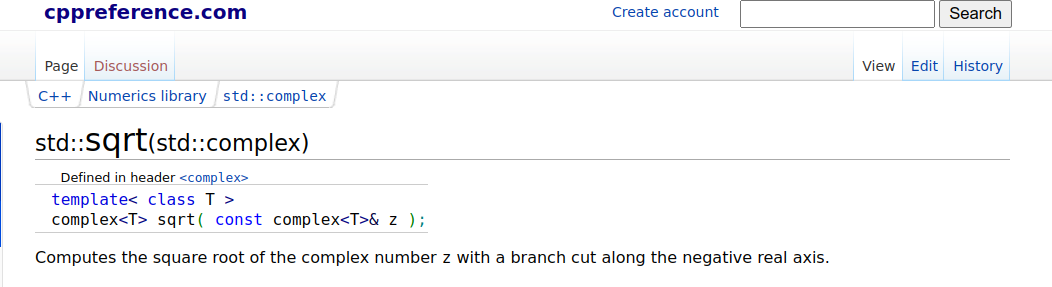
\includegraphics[width=\linewidth]{./gfx/cpp-sqrt-cpp}
	\caption{The article for \texttt{sqrt}, \texttt{sqrtf} and \texttt{sqrtl} in the CPP Reference} \label{fig:cpp-sqrt-cpp}
\end{figure}


\section{External Libraries}
There exists a plethora of libraries that can be used freely in any project to help with common tasks in programming. While these libraries are not part of \enquote{standard C}, some of them are very well known and of outstanding quality. The CPP Reference attempts to collect links to such libraries and lists them under \href{https://en.cppreference.com/w/c/links/libs}{\emph{Non-ANSI/ISO Libraries}} (see \ref{fig:cpp-home}). Using such libraries usually requires you to have a good grasp of the C programming language, so you should only explore that section of the page after you've finished our course. However, once you feel familiar with the core concepts of programming in C, you are bound to find tons of useful tools, for example for games devellopment, linear algebra, networking, ...




\newpage
\section{Exercises and Solutions}
\subsection*{Compiler Invokation}
How do you compile the following piece of code?
\begin{codebox}[exo6-1.c]
\begin{minted}[linenos]{c}
#include <stdio.h>
#include <math.h>

int main () {
   int var;

   printf("please enter an integer: ");
   scanf("%d", &var);

   var = abs(var);

   if (var == 0) {printf("%d has one digit.\n", var);}
   else          {printf("%d has %d digits.\n", var, (int) log10(var) + 1);}
}
\end{minted}
\end{codebox}
What do the functions \texttt{abs} and \texttt{log10} compute?

\subsection*{Modulus for Floating Point Numbers}
You know about the modulus operator \texttt{\%}. Unfortunately, this operator cannot be used with floating point numbers. Find out the function that gives the remainder of a floating point division.

\subsection*{Dice Roll}
Write a program that simulates rolling a die. (Hint: search for \emph{random})\\
Bonus: How do you make sure you do not produce the same number every time you run your program?


\newpage


\subsection*{Solution: Compiler Invocation}
\begin{cmdbox}[Compiling exo6-1.c]
\begin{minted}{text}
gcc -std=c17 -Wall -Wextra -Wpedantic exo6-1.c -lm
\end{minted}
\end{cmdbox}
Note that the \texttt{-lm} flag needs to be placed \emph{behind} the source code (\texttt{exo6-1.c}). You need this flag, because we are using functions from the maths library, as can be seen from line 2 (\texttt{\#include <math.h>}.

In particular, we are using the functions \texttt{abs} (computes the absolute value, \ie makes sure a value is positive) and \texttt{log10} (computes the logarithm to base 10, as opposed to \texttt{log}, which computes the natural logarithm, base $2.718...$).

For details, see \url{https://en.cppreference.com/w/c/numeric/math/abs} and \url{https://en.cppreference.com/w/c/numeric/math/log10}.

\subsection*{Solution: Modulus for Floating Point Numbers}
Typing \enquote{modulus floating point} in the search bar should quickly lead you to \url{https://en.cppreference.com/w/c/numeric/math/fmod} or \url{https://en.cppreference.com/w/c/numeric/math/remainder}. That means, both \texttt{fmod} and \texttt{remainder} are valid answers to the question posed in this exercise. You might also have found the sole difference between the two functions:
\begin{quote}
\emph{In contrast to fmod(), the returned value is not guaranteed to have the same sign as x.}
\end{quote}

\subsection*{Dice Roll}
You should have found the article \url{https://en.cppreference.com/w/c/numeric/random/rand}. With this, you can write this minimal example:

\begin{codebox}[exo6-3a.c]
\begin{minted}[linenos]{c}
#include <stdio.h>
#include <stdlib.h>

int main () {
   printf("The die shows %d pips.\n", rand() % 6 + 1);
   printf("A second roll gives %d pips.\n", rand() % 6 + 1);
}
\end{minted}
\end{codebox}

This does indeed generate a \emph{pseudo}random number. What does \emph{pseudo}random mean?

A computer is a \emph{deterministic} machine, which means it is inherently incapable of producing random results. However, there are functions that behave very erratically. If you have two numbers $x_1$ and $x_2$ and a function $f$, then $f(x_1)$ and $f(x_2)$ may be very different numbers, even if $x_1$ and $x_2$ are very close. With such a function, you can define a recursive sequence: $x_{n+1} = f(x_n)$, \ie you feed the last result of your function back into it to generate the next pseudorandom number.

\texttt{rand} is exactly such a function that behaves so erratically that, for a human, the produced output seems random\footnote{
The function behind this has the form $x_{n+1} = (a x_n + c)\mod m$. The parameters $a$, $c$ and $m$ depend on the specific implementation of the compiler. In case of the \texttt{gcc}, they are $a = 1103515245$, $c = 12345$ and $m = 2^{31}$. See also \url{https://en.wikipedia.org/wiki/Linear_congruential_generator}.
}.

The problem with this method is that, given the same initial value $x_0$, you will always produce the same sequence of pseudorandom numbers. For example, the above code will always produce the output:
\begin{cmdbox}[Output: exo6-3a.c]
\begin{minted}{text}
The die shows 2 pips.
A second roll gives 5 pips.
\end{minted}
\end{cmdbox}

The idea of setting the first value $x_0$ into the pseudorandom number generator is called \emph{seeding}. For this, you can use the function \texttt{srand}, which is mentioned in the article for \texttt{rand} and appears in the example shown there. Maybe you've also noticed the line in the example:
\mint{c}{srand(time(NULL)); // use current time as seed for random generator}

The function \texttt{time(NULL)} returns the number of seconds since a given reference point\footnote{Usually 1970-01-01, 00:00, also known as \emph{The Linux Epoch Time}.}. Unless you can control the flow of time, the result of your program can be seen as random if you seed the pseudorandom number generator with this value.

So, we can add a mere two lines of code to be able to do a \emph{decent} simulation of a dice roll.
\begin{codebox}[exo6-3a.c]
\begin{minted}[linenos]{c}
#include <stdio.h>
#include <stdlib.h>
#include <time.h>

int main () {
   srand(time(NULL));
   
   printf("The die shows %d pips.\n", (rand() + 1) % 6 + 1);
   printf("A second roll gives %d pips.\n", (rand() + 1) % 6 + 1);
}
\end{minted}
\end{codebox}

Maybe you've noticed that in the online example, the dice roll is computed like this:
\mint{c}{x = 1 + rand() / ((RAND_MAX + 1u) / 6); // Note: 1+rand()%6 is biased}
and in particular that they warn against a bias in this evaluation. The remark is correct; however, the \emph{linear congruential generator} (\ie the function behind \texttt{rand}) already has some issues when it comes to statistics. For a simple game, the above method is perfectly fine. If you are doing serious scientific simulations, you should rather not use the function \texttt{rand} at all. The \emph{Gnu Sicentific Library} contains a better pseudorandom number generator. See \url{https://www.gnu.org/software/gsl/} if you're interested -- after learning the basics of programming in C.